\documentclass[12pt,twoside, a4paper, twocolumn]{article}
\usepackage[utf8]{inputenc}
\usepackage[brazil]{babel}
\usepackage[margin = 0.5in]{geometry}
\usepackage{amsmath}
\usepackage{amsthm}
\usepackage{amssymb}
\usepackage{amsthm}
\usepackage{setspace}
\usepackage[americanvoltages,fulldiodes,siunitx]{circuitikz}
\usepackage{lipsum}
\usepackage{pgfplots}
\usepackage{ifthen}
\usepackage{adjustbox}
\usepackage[section]{placeins}
\usepackage{hyperref}
\usepackage{graphicx}
\usepackage{amsmath}
\usepackage{amsthm}
\usepackage{amssymb}
\usepackage{amsthm}
\usepackage{setspace}
\usepackage[americanvoltages,fulldiodes,siunitx]{circuitikz}
\usepackage{lipsum}
\usepackage{pgfplots}
\usepackage{ifthen}
\usepackage{adjustbox}
\usepackage[section]{placeins}
\usepackage{hyperref}
\usepackage{graphicx}
\usepackage{adjustbox}
\usepackage{indentfirst}


\pgfplotsset{compat=newest}
\graphicspath{ {./images/} }
%  #1 color - optional #2 x_0 #3 y_0 #4 x_f #5 y_f #6 name - optional  #7 true if adding lines to axis
\newcommand{\drawvector} [9] [color=cyan] {
\draw[line width=1.5pt,#1,-stealth](axis cs: #2, #3)--(axis cs: #4, #5) node[anchor=south west]{$#6$};
\ifthenelse{\equal{#7}{true}}{
\draw[line width=1pt,#1, dashed](axis cs: #4, #5)--(axis cs: #4, 0) node[anchor= north west]{$#8$};
\draw[line width=1pt,#1, dashed](axis cs: #4, #5)--(axis cs: 0, #5) node[anchor=south east]{$#9$};
}
{}
}
\newcommand\deriv[2]{\frac{\mathrm d #1}{\mathrm d #2}}
\title{Quinto Relatório de Lab de Circuitos II}
\author{Henrique da Silva \\ hpsilva@proton.me}
\date{\today}
\pgfplotsset{width = 10cm, compat = 1.9}
\begin{document}
\maketitle
\pagenumbering{gobble}
\newpage
%pagenumbering{roman}
\tableofcontents
\newpage




\section{Introdução}


Neste relatório, vamos discutir filtros de Butterworth, em particular, vamos projetar, montar e testar um filtro de Butterworth ativo passa-baixa de quarta ordem.


Todos arquivos utilizados para criar este relatório, e o relatorio em si estão em:  \url{https://github.com/Shapis/ufpe_ee/tree/main/5th semester/Circuits II/}


\section{Análise preliminar}


Utilizarei o Maxima para fazer a análise teórica do circuito antes de montá-lo fisicamente.


Após terminar as análises compararei os resultados obtidos nas análises numéricas e em laboratório para verificar sua coerência.


\subsection{O circuito}


\begin{figure}[h]
    \centering
    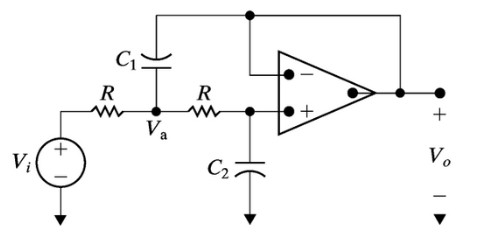
\includegraphics[width=1\columnwidth]{images/circuito.png}
    \caption{Filtro ativo Butterworth de segunda ordem.}
\end{figure}


\pagebreak


\subsection{Maxima}


Podemos realizar a análise do circuito utilizando análise nodal.




\begin{equation}
    \begin{aligned}
         & \frac{V_a - V_i}{R} + \left(V_a - V_o\right) s C1 + \frac{V_a - V_o}{R} = 0 \\
         & \frac{V_o - V_a}{R_2} + V_o s C_2 = 0
    \end{aligned}
\end{equation}


Resolvendo simbolicamente no Maxima obtemos o seguinte:


\begin{equation}
    \frac{\frac{1}{C_1 C_2 R^2}}{s^2 + \frac{2s}{C_1 R} + \frac{1}{C_1 C_2 R^2}}
\end{equation}


Daqui vemos que temos um circuito passa-baixa com os seguintes parâmetros:


\begin{equation}
    \begin{aligned}
         & \omega_c^2 = \frac{1}{C_1 C_2 R^2} \\
         & \beta = \frac{2}{C_1 R}
    \end{aligned}
\end{equation}


E já que estamos tratando de um filtro Butterworth de quarta ordem, precisamos analisar as projeções das raízes dos seus pólos no eixo real.


No caso, só observamos as do segundo quadrante, já que as suas projeções são iguais às das raízes que se encontram no terceiro quadrante.


\begin{equation}
    \begin{aligned}
         & \beta_1 = 2 \left| \cos{\frac{5 \pi}{8}} \right| = 0.765367 \\
         & \beta_2 = 2 \left| \cos{\frac{7 \pi}{8}}\right| = 1.847759  \\
    \end{aligned}
\end{equation}


Com esta informação podemos projetar os filtros protótipos que utilizaremos em série para obter nosso filtro de quarta ordem.


\subsubsection{Filtro 1}


Neste filtro chamaremos seus resistores de $R_1$ seus capacitores de $C_1$ e $C_2$.


\begin{equation}
    \begin{aligned}
         & \beta_1 = 0.765367 = \frac{2}{C_1 R}   \\
         & \omega_c^2 = 1 = \frac{1}{C_1 C_2 R^2} \\
         & R = 1;
    \end{aligned}
\end{equation}


Resolvendo para essas equações teremos:


\begin{equation}
    \begin{aligned}
         & R_1 = 1 \varOmega \\
         & C_1 = 2.6131 F    \\
         & C_2 = 0.38268 F
    \end{aligned}
\end{equation}


Agora vamos realizar o escalonamento para $50Hz$, já que o nosso circuito protótipo foi projetado para $1Hz$.


Utilizaremos as seguintes equaçoes de escalonamento:


\begin{equation}
    \begin{aligned}
        R' = R  k_m \\
        C' = \frac{C}{k_m k_f}
    \end{aligned}
\end{equation}


Com $k_f = 50$ para escalonarmos a frequência central para $50Hz$ e escolhemos um valor de $k_m = 8.3 * 10^4$ para utilizarmos apenas um único resistor com valor comercial.


Então obteremos os seguintes componentes que serão usados para montar o filtro:


\begin{equation}
    \begin{aligned}
         & R_1 = 83k \varOmega \\
         & C_1 = 100 nF        \\
         & C_2 = 14.7 nF
    \end{aligned}
\end{equation}




\subsubsection{Filtro 2}


Neste filtro chamaremos seus resistores de $R_2$ seus capacitores de $C_3$ e $C_4$.


\begin{equation}
    \begin{aligned}
         & \beta_2 = 1.847759 = \frac{2}{C_3 R}   \\
         & \omega_c^2 = 1 = \frac{1}{C_3 C_4 R^2} \\
         & R = 1;
    \end{aligned}
\end{equation}


Resolvendo para essas equações teremos:


\begin{equation}
    \begin{aligned}
         & R_2 = 1 \varOmega \\
         & C_3 = 1.08239 F   \\
         & C_4 = 0.92388 F
    \end{aligned}
\end{equation}


Agora vamos realizar o escalonamento para $50Hz$, já que o nosso circuito protótipo foi projetado para $1Hz$.


Utilizaremos as seguintes equaçoes de escalonamento:


\begin{equation}
    \begin{aligned}
        R' = R  k_m \\
        C' = \frac{C}{k_m k_f}
    \end{aligned}
\end{equation}


Com $k_f = 50$ para escalonarmos a frequência central para $50Hz$ e escolhemos um valor de $k_m = 6.2 * 10^4$ para utilizarmos apenas um único resistor com valor comercial.


Então obteremos os seguintes componentes que serão usados para montar o filtro:


\begin{equation}
    \begin{aligned}
         & R_2 = 62k \varOmega \\
         & C_3 = 55.6 nF       \\
         & C_4 = 47.4 nF
    \end{aligned}
\end{equation}


\subsubsection{Filtro combinado}


Podemos então combinar os dois filtros de Butterworth de segunda ordem que projetamos em série para obter um filtro de quarta ordem com a seguinte função de transferência:


\begin{equation}
    \begin{aligned}
         & H(s) = \frac{\omega_c^4}{\left( s^2 + \beta_1 s + \omega_c^2 \right) \left( s^2 + \beta_2 s + \omega_c^2 \right)} \\
         & \beta_1 = 0.765367                                                                                                \\
         & \beta_2 = 1.847759                                                                                                \\
         & \omega_c = 2 \pi 50 = 314.159265                                                                                  \\
    \end{aligned}
\end{equation}




\subsubsection{Gráfico de Bode}


\begin{figure}[h]
    \centering
    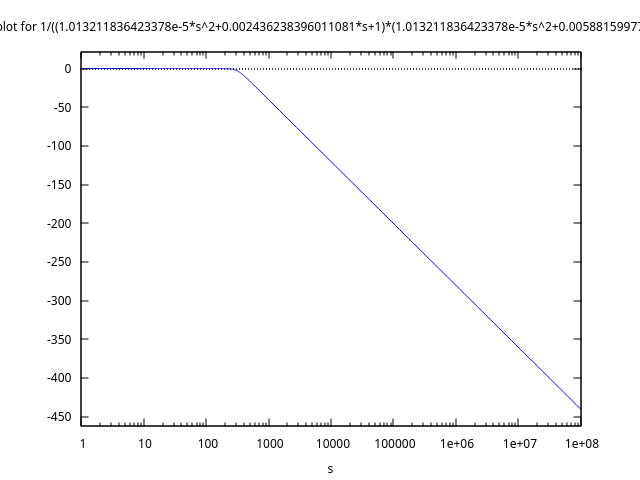
\includegraphics[width=1\columnwidth]{images/bodegain.png}
    \caption{Magnitude de H(s) do filtro.}
\end{figure}


Temos $80dB$ de perda em $500Hz$ e $160dB$ de perda em $5000Hz$.


Cada filtro de Butterworth tem $40dB$ de perda por década. Como temos dois em série, perdemos $80dB$ por década.


Em outras palavras, temos $20dB$ de perda por polo por década. Como temos 4 polos, perdemos $80dB$ por década.


Então o que observamos é coerente.


\pagebreak


\section{Medições em laboratório}




\subsection{Os filtros}


Inicialmente farei as medições dos componentes a serem usados.


Após isso farei um breve teste em cada um dos filtros de segunda ordem individualmente.


Por fim, combinarei os dois filtros no nosso filtro de quarta  ordem que queremos analisar.


\subsection{Tabela de componentes}


\subsubsection*{Filtro 1}
\begin{equation}
    \begin{aligned}
        R_1 & = 81.1k \varOmega \\
        R_2 & = 81k \varOmega   \\
        C_1 & = 100 nF          \\
        C_2 & = 14.7 nF         \\
    \end{aligned}
\end{equation}


\subsubsection*{Filtro 2}
\begin{equation}
    \begin{aligned}
        R_3 & = 61.8k \varOmega \\
        R_4 & = 61.2k \varOmega \\
        C_3 & = 55.5 nF         \\
        C_4 & = 47.8 nF         \\
    \end{aligned}
\end{equation}


\subsection{Gráficos de Bode dos filtros reais}


Substitui os valores reais no Maxima para obter gráficos de Bode dos filtros reais. Para observar o comportamento real esperado.


\subsubsection{Filtro 1}


\begin{figure}[h]
    \centering
    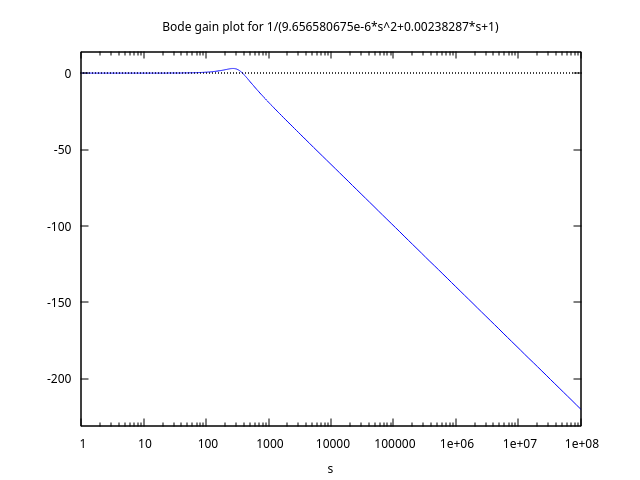
\includegraphics[width=1\columnwidth]{images/bodegainH1.png}
    \caption{Magnitude de H(s) do filtro 1.}
\end{figure}


Notamos que há um ganho considerável antes de começar a filtrar frequências altas.


Achamos uma frequência de corte de $71Hz$.


\subsubsection{Filtro 2}


\begin{figure}[htbp!]
    \centering
    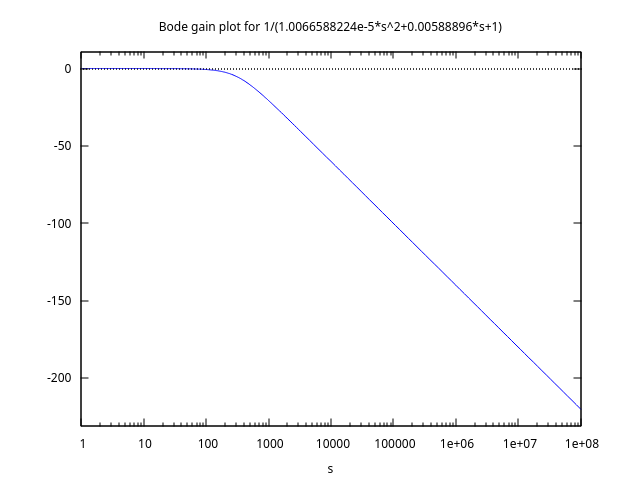
\includegraphics[width=1\columnwidth]{images/bodegainH2.png}
    \caption{Magnitude de H(s) do filtro 2.}
\end{figure}


Achamos uma frequência de corte de $36Hz$.


\subsubsection{Filtro total}


\begin{figure}[htbp!]
    \centering
    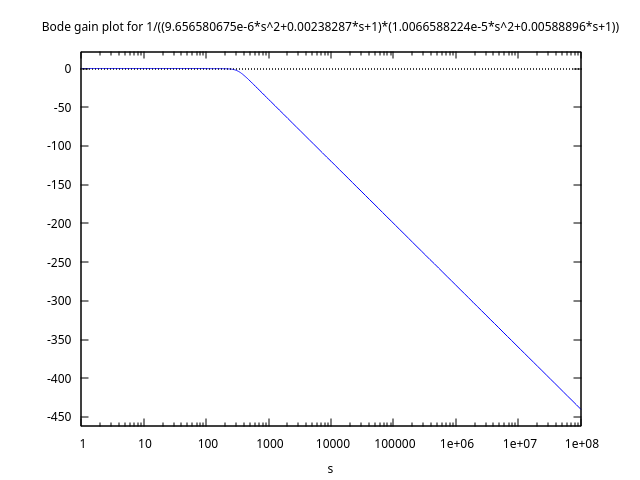
\includegraphics[width=1\columnwidth]{images/bodegainHtotal.png}
    \caption{Magnitude de H(s) do filtro total.}
\end{figure}


Achamos uma frequência de corte de $50Hz$.




\pagebreak






\subsection{Comportamento na frequência}


Em frequências baixas constatamos que o ganho permanecia 1. E achamos sua frequência de corte de fato em 59Hz. Como esperávamos da análise numérica com os valores reais.


Notamos também que há um pequeno ganho antes de atingirmos a frequência de corte. Este comportamento pode ser observado no gráfico de Bode do filtro 1 que fizemos acima na seção (3.3.1).


As fotos do osciloscópio se encontram na pasta do relatório em "images/osciloscopio/*".




\subsection{Resultados das medidas}
\begin{center}
    \begin{tabular}{ |c|c|c|c| }
        \hline
        Múltiplos & Freq (Hz) & Entrada (V) & Saída (V) \\
        0.25      & $14.75$   & $5.11$      & $5.15$    \\
        0.5       & $29.5$    & $5.11$      & $5.47$    \\
        0.75      & $44.25$   & $5.11$      & $5.39$    \\
        1         & $59$      & $5.11$      & $3.62$    \\
        1.25      & $73.75$   & $5.11$      & $2.01$    \\
        1.6       & $94.4$    & $5.11$      & $0.97$    \\
        2.5       & $147.5$   & $5.11$      & $0.3$     \\
        \hline
    \end{tabular}
\end{center}




\newpage




\section{Pós-laboratorial}


As tabelas estão na seção 3.2 e 3.5.


\subsection{Função transferência de todos filtros envolvidos.}


\subsubsection{Filtro 1}


\begin{figure}[h]
    \centering
    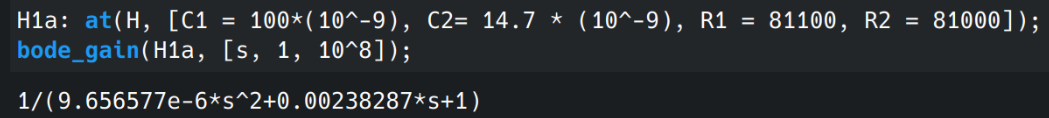
\includegraphics[width=1\columnwidth]{images/hsfiltro1.png}
    \caption{H(s) do filtro 1 com valores reais.}
\end{figure}


\begin{figure}[h]
    \centering
    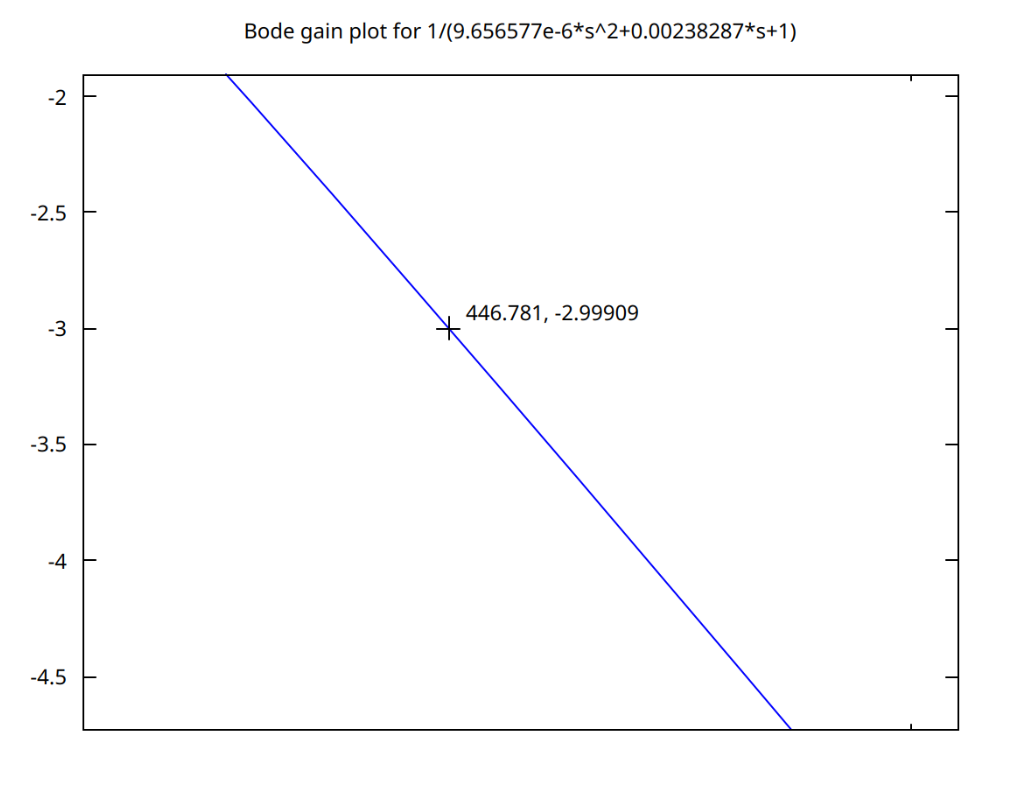
\includegraphics[width=1\columnwidth]{images/zoomH1.png}
    \caption{Zoom do gráfico de Bode do filtro 1 com valores reais.}
\end{figure}


Daqui tiramos uma frequência de corte de $71.1Hz$ a partir do gráfico de Bode desta função.




\subsubsection{Filtro 2}


\begin{figure}[h]
    \centering
    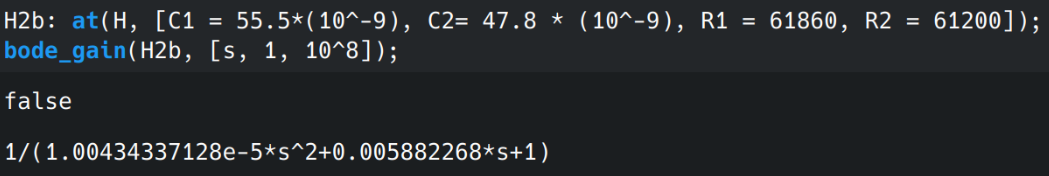
\includegraphics[width=1\columnwidth]{images/hsfiltro2.png}
    \caption{H(s) do filtro 2 com valores reais.}
\end{figure}


\begin{figure}[h]
    \centering
    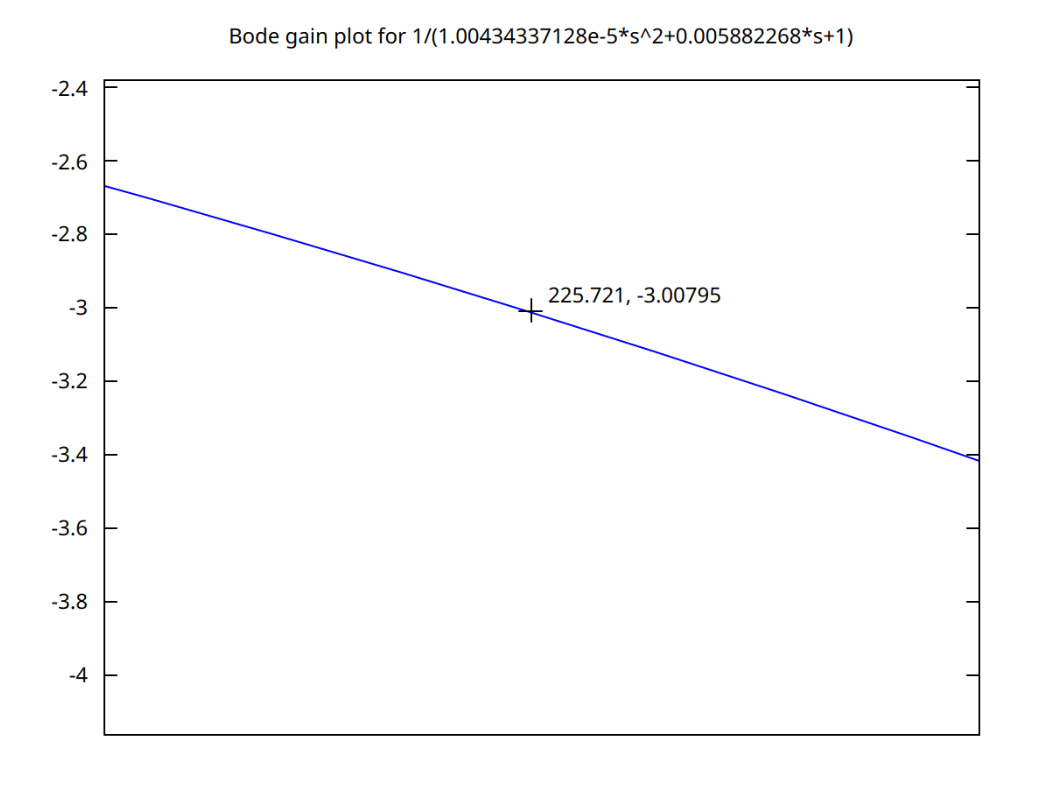
\includegraphics[width=1\columnwidth]{images/zoomH2.png}
    \caption{Zoom do gráfico de Bode do filtro 2 com valores reais.}
\end{figure}


Daqui tiramos uma frequência de corte de $35.9Hz$ a partir do gráfico de Bode desta função.




\pagebreak
\subsubsection{Filtro total}


\begin{figure}[htbp!]
    \centering
    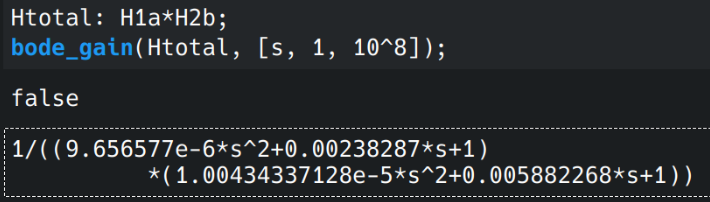
\includegraphics[width=1\columnwidth]{images/hsfiltrototal.png}
    \caption{H(s) do filtro total com valores reais.}
\end{figure}


\begin{figure}[htbp!]
    \centering
    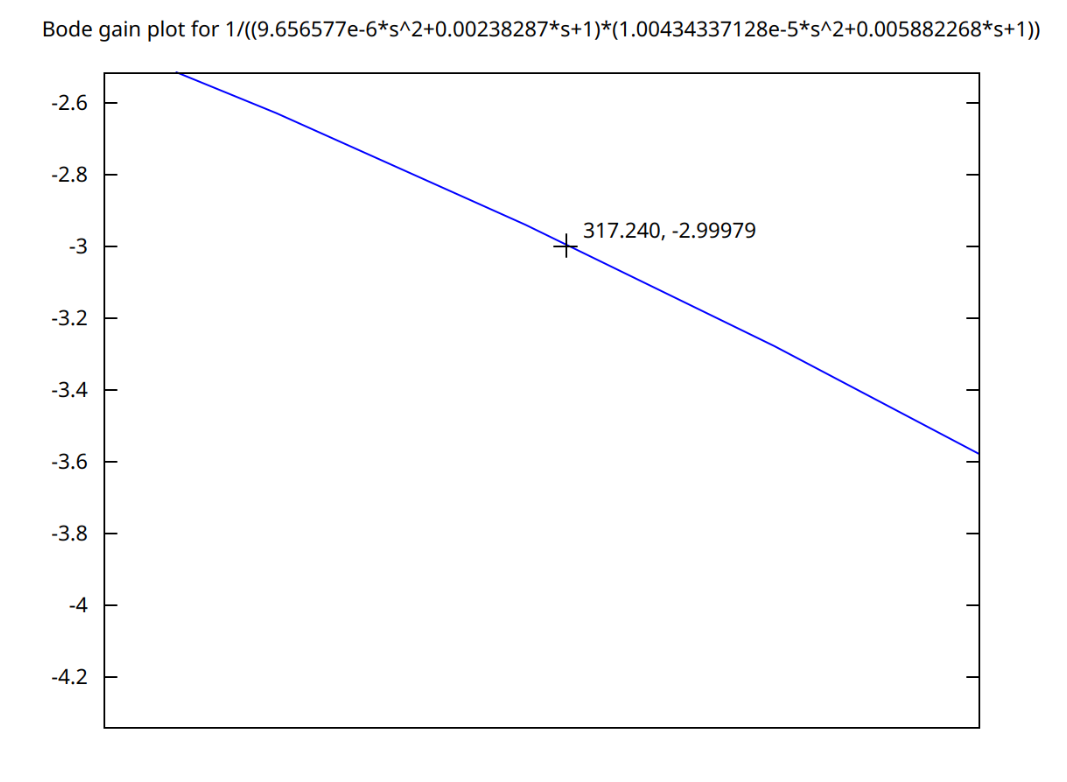
\includegraphics[width=1\columnwidth]{images/zoomHtotal.png}
    \caption{Zoom do gráfico de Bode do filtro total com valores reais.}
\end{figure}


Daqui tiramos uma frequência de corte de $50.5Hz$ a partir do gráfico de Bode desta função.




\pagebreak


\subsection{Ganho do filtro}


Observamos um ganho unitário, que ocorre quando $s = jw$ com $w$ tendendo a $0$.


Que é o resultado esperado para filtro passa-baixa.




\subsection{Tabela de magnitudes}


\begin{center}
    \begin{tabular}{ |c|c|c|c| }
        \hline
        Múltiplos & Freq (Hz) & $\left| H(jw) \right|$ \\
        0.25      & $14.75$   & $1.0078$               \\
        0.5       & $29.5$    & $1.0704$               \\
        0.75      & $44.25$   & $1.0547$               \\
        1         & $59$      & $0.7084$               \\
        1.25      & $73.75$   & $0.3933$               \\
        1.6       & $94.4$    & $0.1898$               \\
        2.5       & $147.5$   & $0.0587$               \\
        \hline
    \end{tabular}
\end{center}


\subsection{Dados achado e gráfico de Bode}


\begin{figure}[h]
    \centering
    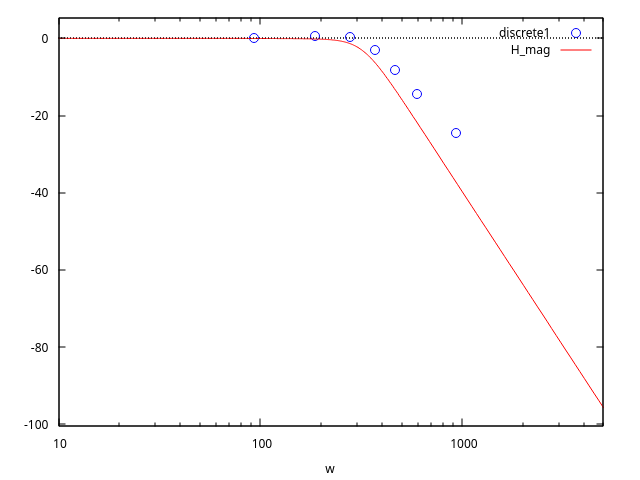
\includegraphics[width=1\columnwidth]{images/magnitudepontosreais.png}
    \caption{Gráfico da curva esperada pelos pontos encontrados.}
\end{figure}


Há uma discrepância, que já havíamos detectado. Em 4.1.3 vimos que a frequência de corte esperada com os valores reais dos componentes eh de $50.5Hz$, e a que encontramos experimentalmente foi de $59Hz$.


Eu não tenho certeza de por que houve essa discrepancia. Creio que seja por conta de erro de medição dos valores dos componentes.


\newpage




\section{Conclusões}


Conseguimos com sucesso fazer a análise numérica pelo Maxima, e comparamos os resultados com os obtidos experimentalmente.


Nos resultados práticos, a magnitude da função transferência e as frequências de corte foram coerentes com os resultados esperados.


Porém, houve o erro evidenciado em 4.3, de que a frequência de corte esperada pelos valores de componentes medidos era de $50.5Hz$, e a que de fato achamos foi de $59Hz$.


Creio que por conta de erro de medição dos valores dos componentes.


Os gráficos que geramos a partir dos resultados experimentais foram coerentes com os gráficos gerados numericamente.


Em suma creio que tivemos sucesso em nos familiarizar com as ferramentas de análise de circuitos elétricos numéricos.


\end{document}